\chapter{ソフトウェア・パッケージIvyの開発}
\section{研究背景}
RNA-seqデータを対象としたRNA編集サイトの検出ソフトウェアは、REDITools \citep{Picardi:2013aa}一つの実装に限られている。そのため、SNPやSNVをDNA-seqデータから検出する変異解析用のソフトウェアとして開発されているsamtools mpileup \citep{Li:2009aa}、GATK \citep{McKenna:2010aa}、SOAPsnp \citep{Yu:2013aa}転用した研究例も複数がある \citep{Danecek:2012aa, Chen:2012aa, Sanjana:2012aa, Peng:2012aa}。これは、RNA編集サイトもSNP/SNVの検出も本質的にはショートリードのマッピング結果からゲノム配列との一塩基変異を検出することにほかならないからである。しかしながら、DNA-seqとRNA-seqのアラインメント結果を観察すると、一般にRNA-seqデータはDNA-seqに対して数百倍の変異箇所が見られる。これは、第1章や2章で述べたように、RNA分子の不安定性や複数のマッピングバイアスが影響しているからである。こういった現状において、一つのソフトウェアでRNA編集サイトの検出が完結した例はこれまでにない。一般的には、実験で得られたRNA-seqデータを参照ゲノム配列へ適切なパラメータでマッピングし、そのアラインメントについて数個から多い時には20以上のフィルタリングを通し、最終的にそれらのフィルタリングを通過した箇所をRNA編集サイトとしてリストする、という方法が取られる。変異解析のソフトウェアを用いた場合でも、下流解析では独自のフィルタリング過程を必ず設け、擬陽性を減少させる工夫が行われている。そのため、必然的に情報解析のワークフローは複数のフィルタリングと条件分岐によって複雑化する。
\par
超並列シーケンスデータを用いたRNA編集サイトの検出には、現在二つの問題がある。一つ目は、高精度な検出のために解析が複雑化し、簡便かつ高速な解析が困難となっていることである。第\ref{bench}章の精度検証の対象となった検出手法もまたその例外ではなく、使用したソフトウェアや解析方法の詳細なパラメータに関しては、自然言語によって論文中では記述される。そのため、論文ごとに解析手法の記述には粒度の違いが見られ、完全な再現が困難な場合もある。こういった現状では、仮に先行研究ごとにシーケンスデータが公開されていたとしても、複雑な解析パイプラインを再現し、優れた手法を他のデータへ適用することや、追証実験を行い難いという問題を発生させる。二つ目の問題は、新規の検出手法によって編集サイトを検出した場合に、検出精度の検証方法がばらつき、手法やパラメータの影響についての比較検討が困難だということである。第2章では、検出手法の精度比較を主題とし、情報検索の分野で利用されてきた適合率や再現率の導入による解決方法の提案を試みたものであった。
\par
本研究では、上記二つの問題を解決するため、超並列シーケンスデータを対象としたRNA編集サイトの高速かつ高精度な検出に加え、精度検証を行うソフトウェア・パッケージIvyの開発を目的として、研究を行った。Ivyはコマンドラインツールとして実装され、RNA編集サイトを検出するためのツールと精度検証を行うためのベンチマークツールが付属されたパッケージとなっている。尚、GNU GPLv3 (GNU General Public License version 3)の元、オープンソースのフリーウェアとして、\url{http://}において公開する予定である。
\par
結果、既存のソフトウェアならびに変異解析で用いられるソフトウェアよりも高速かつ低メモリで動作することが示された。

\section{システムの設計}
\subsection{動作環境}
IvyはUnix環境で動作するコマンドラインツールとしてPython v2.7.5によって実装された。図\ref{fig:ivy_arch}には、Ivyシステムの設計の
全体像を示した。Ivyのシステムは、オブジェクト指向プログラミングによる開発を取り入れており、適切なクラス設計によりユーザーとなる研究者からの追加機能の要望にも柔軟に対応できるような拡張性の高い実装を実現している。Ivyは、RNA編集サイトを検出するためのivyと、精度検証を行うためのedit\_benchの二つのコマンドラインツールが独立して動作する。
\par
Ivyの開発は、Mac OSX 10.9上のPython v.2.7.5で行われており、Python3およびそれ以下のバージョンでは動作試験は行っていない。Mac以外のUnix環境として、RedHat上での動作は確認している。ivyは、入力として受け取るアラインメントデータの処理にはPysam v0.7.5、VCF (Variant call format) \citep{Danecek:2011aa}の処理にはpyVCF v0.6.4、高速なフィッシャーの正確確率検定のためのfisher v0.1.4に依存する。edit\_bechは、図の生成にmatplotlib v1.4.1+に依存する。これらの依存関係は、インストール時に自動的に解決を試みる仕様だが、高速化のために一部のライブラリのインストールには、事前にCコンパイラを用意しておく必要がある。インストール自体はコマンド一つで簡便に行えるようになっているほか、PyPI (Python package index)への登録を予定しており、インストール時にソースコードのダウンロードも不要となる予定である。

\subsection{ivyの実装}
ivyは、ユーザーから与えられたRNA-seq/DNA-seqのアラインメントファイルと参照ゲノム配列、解析のパラメータを引数として受け取り、動作する。基本的な動作として、受け取った引数からリファレンスゲノムの配列と一塩基ごとにアラインメント結果を解析する。一塩基ごとのアラインメント情報の取得は、ストリーミングで処理され、各種のフィルタリング処理が行われる。設定されたフィルタリングを通過した最終的な候補サイトは、ファイルへと書き出され、ivyによる解析は終了する。以降では、詳細なivyのクラス設計と実装を概観してゆく。
\par
AlignmentStreamクラスは、入力されたバイナリ形式のアラインメントの情報が含まれるオブジェクトを一塩基ごとに読み出す中核的なクラスである。このように参照ゲノムの一塩基ごとにRNA-seq/DNA-seqのアラインメント結果へと変換する過程をpileupと呼び、pileupしたpysam.AlignedRead
オブジェクトは、ショートリードの配列、リードの向きやクオリティ、参照ゲノムへの座標などアラインメント結果に関する多くの属性 (Attributes)を持つ。AlignmentStreamクラスはこれらの属性を参照しながら、委譲 (Deligation)されたAlignmentFilterクラスやAlignmentReadStatsクラスが、アラインメント結果のフィルタリングや統計的なバイアスのフィルタリングを行う実装を持つ。AlignmentStreamでのpileup処理は、数百MBから数十GBのアラインメントファイルを対象とするため、ヒトゲノムの解析では一番染色体へ限定的に解析したとしてもオブジェクトのサイズはメモリ空間を圧迫しかねない。そのため、AlignmentStream.pileup\_streamメソッドは、pileupした返り値をイテレータとする実装を持ち、
省メモリでの解析を実現している。また、ivyはLoggerクラスを持ち、解析の各段階における累積時間、解析に使用された全オプション、発生した警告やエラーの出力などを制御している。ivyが期待と異なった動作をした場合には、Loggerクラスから出力された冗長なログが有用だと考えられる。デフォルトでログの出力レベルは最低限に抑えられており、必要に応じて有効にして使う実装とした。
\par
Ivyは、ヒト、マウス、ショウジョウバエといった高等真核生物を主要な解析対象種とした編集サイトの検出を実行する。原理的には、pileupをするためのメソッドコール数は、ゲノムサイズに完全に比例し、ゲノムサイズが大きな生物に対しては計算時間が増大することが予想される。そのため、複数のスレッドを使用した並列化が現実的な時間内での解析には必須だと考えた。ivyは、pythonの標準ライブラリを使用した並列処理を提供する。検出の高速化のために使用可能なスレッド数に応じ、自動的に染色体数を均等に分割し、編集サイトを検出する。RNA 編集サイトは、染色体をオーバーラップして起こる現象ではないため、染色体を分割することによるアラインメントデータの損失などの問題は起こらないと考えた。

\subsection{edit\_benchの実装}
edit-benchは、検出されたRNA編集サイトの精度検証を行うためのベンチマークツールとして開発された。精度検証には、第2章で用いた再現率、適合率およびF値を用いた。各指標については、第2章を参照されたい。
\par
edit-benchは大きく4つのクラスから実装され、Darnedから正解セットをHTTP通信により取得し、適切なCSVファイルにパースするGeneratorクラス、何らかの方法により検出されたRNA編集サイトのVCFファイルから、適切なデータ構造を生成と読み出しをするReaderクラス、精度検証のための各種指標を計算するBenchmarkクラス、精度の検証結果を図によって可視化するPlotクラスを持つ。Generatorクラスでは、初回起動のみ引数に与えられた生物種名に対応した正解セットをDarnedより取得する必要から時間を要するが、2回目以降はローカルにCSVファイルとしてキャッシュするため高速に動作する。
Readerクラスは、ivyの出力であるVCF (Variant call format)を入力とし、データ構造に保存する他に、検出された編集サイトの個数などの情報を取得するメソッドを持つ。Benchmarkクラスは、Readerクラスによって生成されたデータ構造を利用して、精度検証の指標を計算する。Plotクラスは、再現率と適合率に関する二次元プロットを生成するクラスであり、図の描画は補助的な機能ではなく、精度検証の結果から手法の妥当性を直感的に判断することを可能にしている。この描画機能は、複数回ivyを実行し、最も精度のよいパラメータの組み合わせを得る場合に使用されることを想定する。また、検証を行うサンプル数が多い場合、ラベルの色分けが離散的であると色が飽和する問題があるが、サンプル数に応じてカラーマップから連続的な階調を自動生成することで回避した。描画された結果は、PDFファイルへと出力される。尚、図の生成にはmatplotlibパッケージに依存するが、他のクラスはPythonの組み込みライブラリのみで動作する。
\begin{figure}[!h]
	\begin{center}
		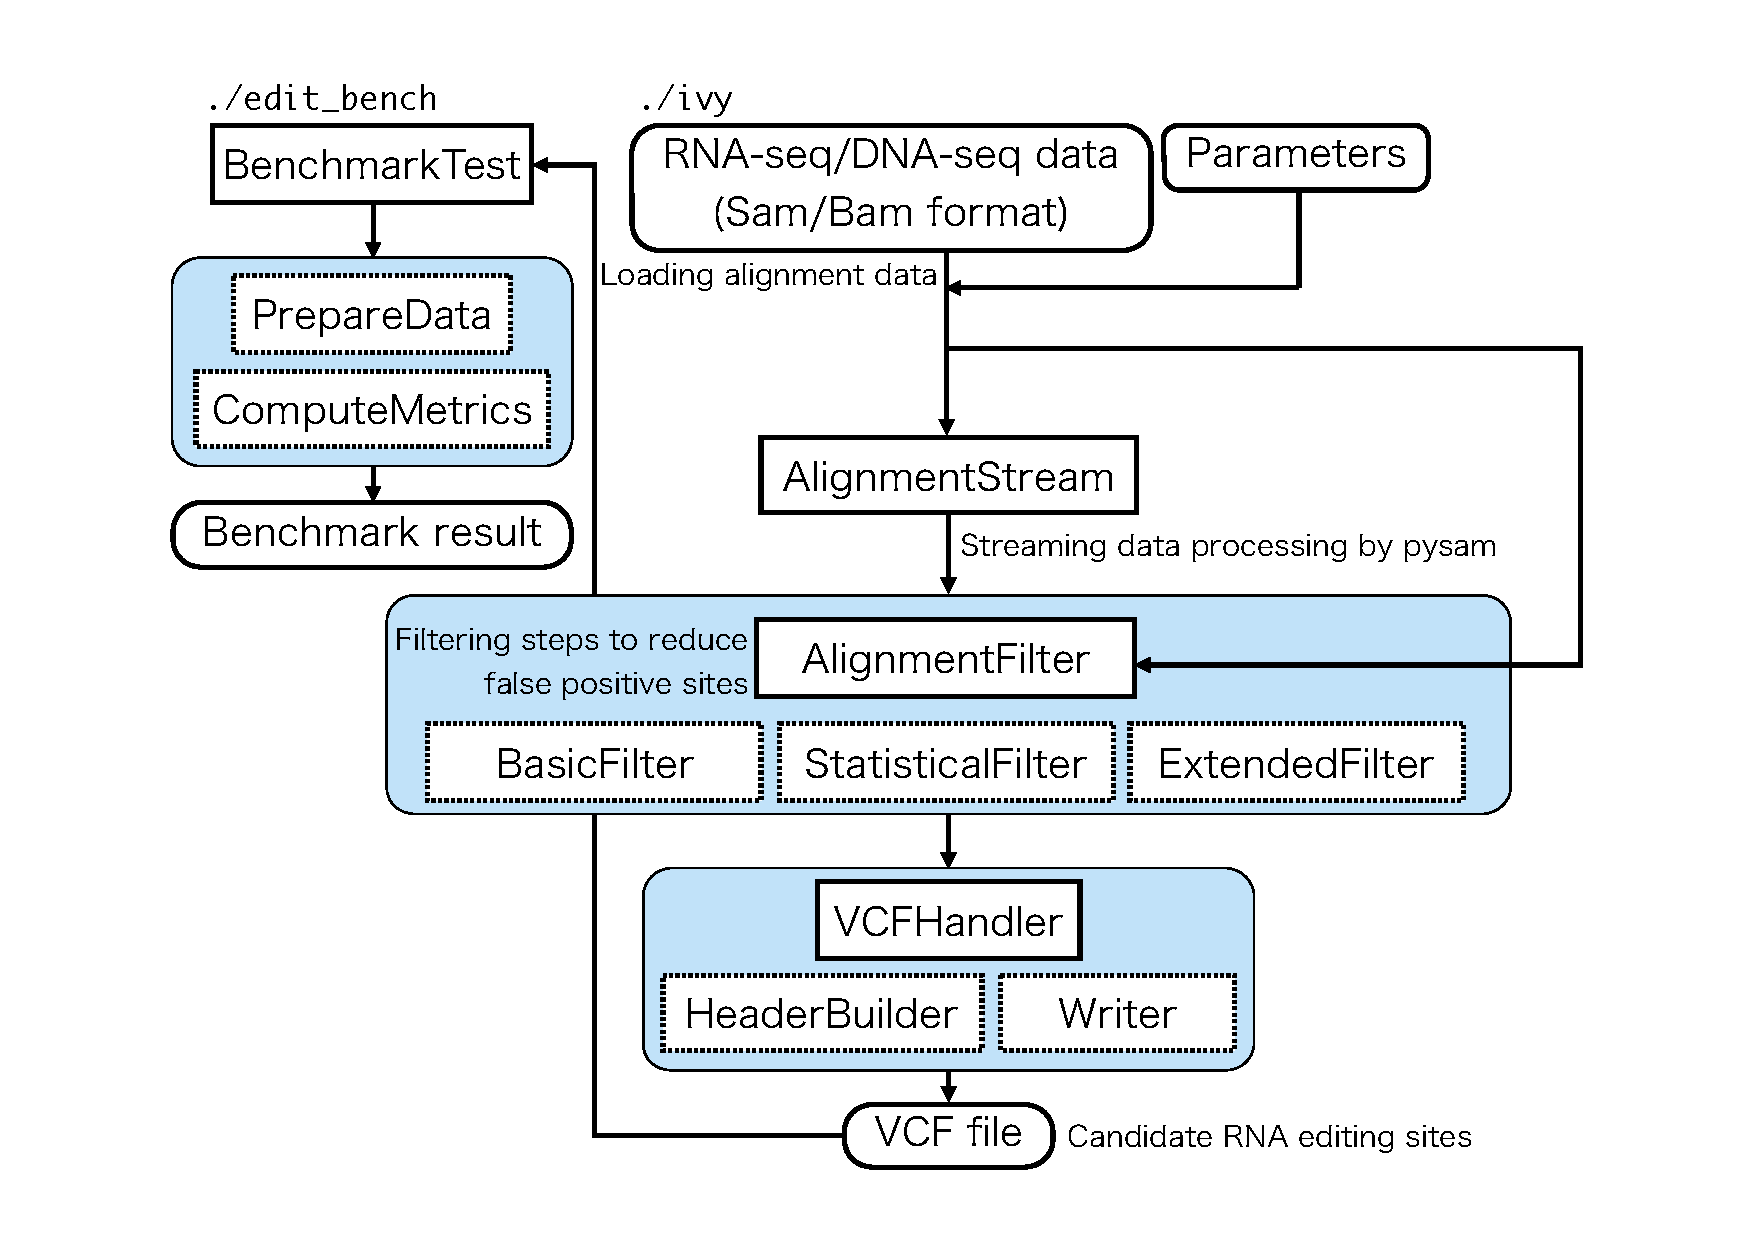
\includegraphics[width=1 \hsize]{ivy_arc.pdf}
	\end{center}
	\vspace*{-1cm}
	\caption{ソフトウェア・パッケージIvyの設計}
	\label{fig:ivy_arch}
	\begin{flushleft}
		\small{設計されたIvyの全体像を示す。ここで示した全体像は、実装を簡略化して示している。矢印は、入力として受け取ったRNA-seq/DNA-seqデータと解析パラメータを受け取り、最終的にRNA編集サイトが検出されるまでの流れを示す。}
	\end{flushleft}
\end{figure}

\subsection{入出力の形式}
超並列シーケンサーを用いた解析において、塩基配列データはFastqフォーマットが標準的な形式となっており、Fastqデータを参照ゲノム配列にマッピングすることによって、SNPの検出や遺伝子発現量の定量、ゲノムのアセンブリなどが行われ、RNA 編集サイトの検出も参照ゲノムへのマッピングが検出には必須である。このマッピングしたアラインメント結果を保持するデータ形式は、SAM/BAM形式が事実上の標準フォーマットとして広く用いられている。SAMは参照ゲノムへマッピングされたショートリードの座標情報やクオリティ情報などを保持しており、座標にインデックスを貼りgzipで圧縮したバイナリ形式をBAMと呼ぶ。SAMとBAMは相互に変換が可能である。入力は、RNA-seq/DNA-seqリードをマッピングした結果から得られる BAM (Binary alignment/map format)形式である。
\par
入力されたBAMファイルは、Pysam (Python interface for the SAM/BAM sequence alignment and mapping format)ライブラリを使用して、リファレンスゲノムへのアラインメント結果の取得に用いている。Pysamは、C言語で書かれたBAMのパーサーライブラリ (Samtools C API)のラッパーであり、内部では直接C言語のAPIを呼び出しているため高速にアラインメント情報を取得可能である。そのため、本ソフトウェア・パッケージでもpysamをメインのライブラリとして使用した。
\par
Ivyによって検出されたA-to-I 編集サイトは、VCF v4.1によって出力される。このVCFフォーマットは、SNPやSNVの検出といった変異解析に標準的に用いられているフォーマットを指し、1000 genomes project など国際プロジェクトでも採用されているデータ形式である。RNA 編集サイトもSNPも本質的にはゲノムのある座標における一塩基置換として表現可能であるから、検出したRNA 編集サイトもVCF形式で出力することが望ましいと考えた。VCFを出力フォーマットとする利点として、変異解析のために開発された他のミドルウェアを組み合わせた更なる解析が可能となる点である。SNP解析では検出したSNPそれぞれの遺伝子名やアミノ酸置換の有無などをAnnovar \citep{Wang:2010aa}とったソフトウェアを用いてアノテーションする場合が多い。Ivyで出力された結果もまたVCFであるから、Annovarなど他のツールと連携させた下流解析を容易に行うことができるという利点を持つ。

\subsection{ユーザーインターフェース}
Ivyパッケージは、以下のコマンドで容易にインストールすることが可能となっている。ivyのインターフェースは以下のようになっており、同梱されているサンプルデータを用いて解析を簡易的に試すことができるようになっている。
\begin{itembox}[l]{Ivyのインストール}
	\begin{verbatim}
		# 最新版のソースコードの取得
		$ curl https://github.com/soh-i/Ivy/archive/master.zip
		# パッケージのインストール
		$ python setup.py install
	\end{verbatim}
\end{itembox}

\subsubsection{ivyコマンドのインターフェース}
\begin{itembox}[l]{\url{ivy}コマンドのインターフェース}
	\begin{verbatim}
		# ヘルプの表示
		$ ivy --help
		# 最も基本的な解析
		$ ivy -f human_hg19.fa -r sample_rna.bam -d sample_dna.bam
	\end{verbatim}
\end{itembox}

\subsubsection{edit\_benchコマンドのインターフェース}
edit\_benchは、以下のようなインターフェースから使用可能である。入力には、検出した編集サイトが記述されたVCFファイルの他に、対応する生物種とそのゲノムバージョンを与えると実行可能である。
\par
示した例では、他に\url{--plot}オプションで結果を図として描画する機能を有効にし、
\url{--log}で保存するファイルを指定している。CSV形式で保存される他、カラムのスキーマなどは付録を参照されたい。尚、このオプションが指定されない場合には、標準出力に結果は出力される。\url{--source}オプションは、Darnedのデータセットから特定のセルラインや組織に限ったサブセットを生成し、それを正解セットとした精度検証を可能にする。デフォルトでは、この機能は無効になっており、Darnedの全ての編集サイトを対象に、精度検証の指標は計算される。以下、edit\_benchコマンドのインターフェースと簡単な解析例を示す。
\par
\begin{itembox}[l]{\url{edit_bench}コマンドのインターフェース}
	\begin{verbatim}
		# 基本的な使い方
		$ edit_bench --vcf test.vcf --sp human_hg19 --plot --log bench.log
		# 正解セットを脳のサンプルに限定する
		$ edit_bench --vcf test.vcf --sp human_hg19 --source brain  
		  --log bench.log
	\end{verbatim}
\end{itembox}

\newpage

\section{本手法の性能評価}
\subsection{性能評価に用いたRNA-seqデータ}
\subsubsection{ヒト}

\begin{longtable}{cccc}
	\vspace{-0.5cm}
	\label{tab:darned}\\
	\caption{PMID: 21960545 ヒトのデータ}\\
	\cline{1-4}
	\textbf{Sample} & \textbf{GSM ID} & \textbf{Cell line} & \textbf{Tissue} \\
	\cline{1-4}
	u87\_adar\_ctrl & GSM693746 & U87MG & Glioblastoma \\
	u87\_adar\_kd & GSM693747 & U87MG & Glioblastoma \\
	\cline{1-4}
	\vspace{-0.8cm}
\end{longtable}
\begin{flushleft}
	\small{Accurate identification of A-to-I RNA editing in human by transcriptome sequencing}
\end{flushleft}

\subsubsection{マウス}
\subsubsection{ショウジョウバエ}
\subsubsection{線虫}
\begin{longtable}{cccc}
	\vspace{-0.5cm}
	\label{tab:darned}\\
	\caption{PMID: 22673872 線虫のデータ}\\
	\cline{1-4}
	\textbf{Sample} & \textbf{GSM ID} & \textbf{Strain} & \textbf{Tissue} \\
	\cline{1-4}
	Wild-type small RNA rep1 & GSM715830 & Wild-type (N2) & Whole worm \\
	Wild-type small RNA rep2& GSM715831 & Wild-type (N2) & Whole worm \\
	Adar1-mutant small RNAs & GSM715832 & adr-1 (tm668) & Whole worm \\
	Adar2-mutant small RNAs & GSM715833  & adr-2 (ok735) & Whole worm \\
	Adar-1 and Adar-2 mutant small RNAs & GSM715834 & adr-1;adr-2 (tm668;ok735) & Whole worm \\
	\cline{1-4}
	\vspace{-0.8cm}
\end{longtable}
\begin{flushleft}
	\small{Effects of ADARs on small RNA processing pathways in \textit{C. elegans}.}
\end{flushleft}

\subsection{使用したパラメータ}

\subsection{性能評価の結果}
\subsubsection{メモリ使用効率}
\begin{figure}[!h]
	\begin{center}
		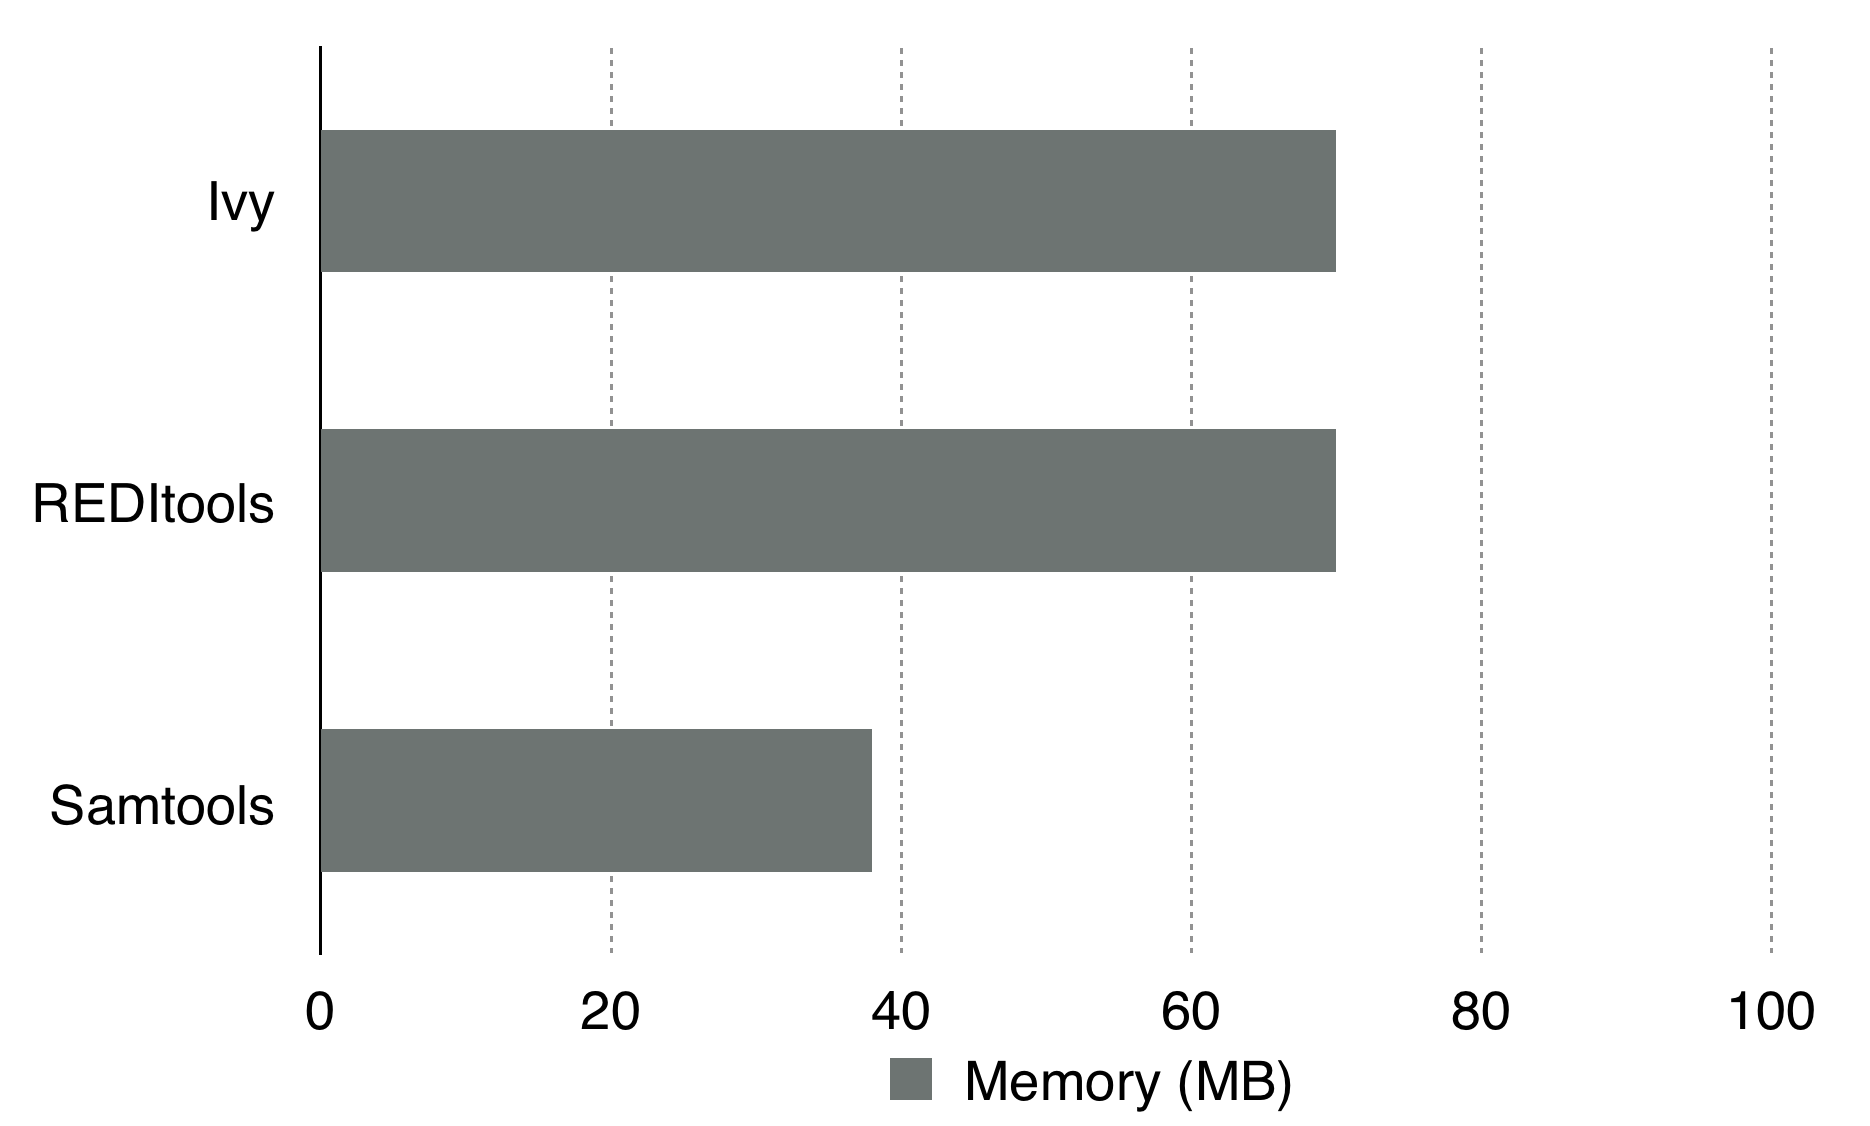
\includegraphics[width=0.7 \hsize]{ivy_memory.png}
	\end{center}
	\caption{メモリの使用効率のベンチマーク}
	\begin{flushleft}
		\small{Ivy、REDItools、samtoolsで比較した。}
	\end{flushleft}
	\label{fig:f_measure}
\end{figure}

\subsubsection{解析に要する累積時間}
\begin{figure}[!h]
	\begin{center}
		\includegraphics[width=0.7 \hsize]{ivy_time.png}
	\end{center}
	\caption{解析時間のベンチマーク (dummy data)}
	\begin{flushleft}
		\small{Ivy、REDItools、samtoolsで比較した。}
	\end{flushleft}
	\label{fig:f_measure}
\end{figure}

\subsection{Ivyの検出精度}
\subsubsection{適合率・再現率による検証}

\subsection{実データを用いたRNA 編集サイトの解析}
\begin{figure}[!ht]
	\begin{center}
		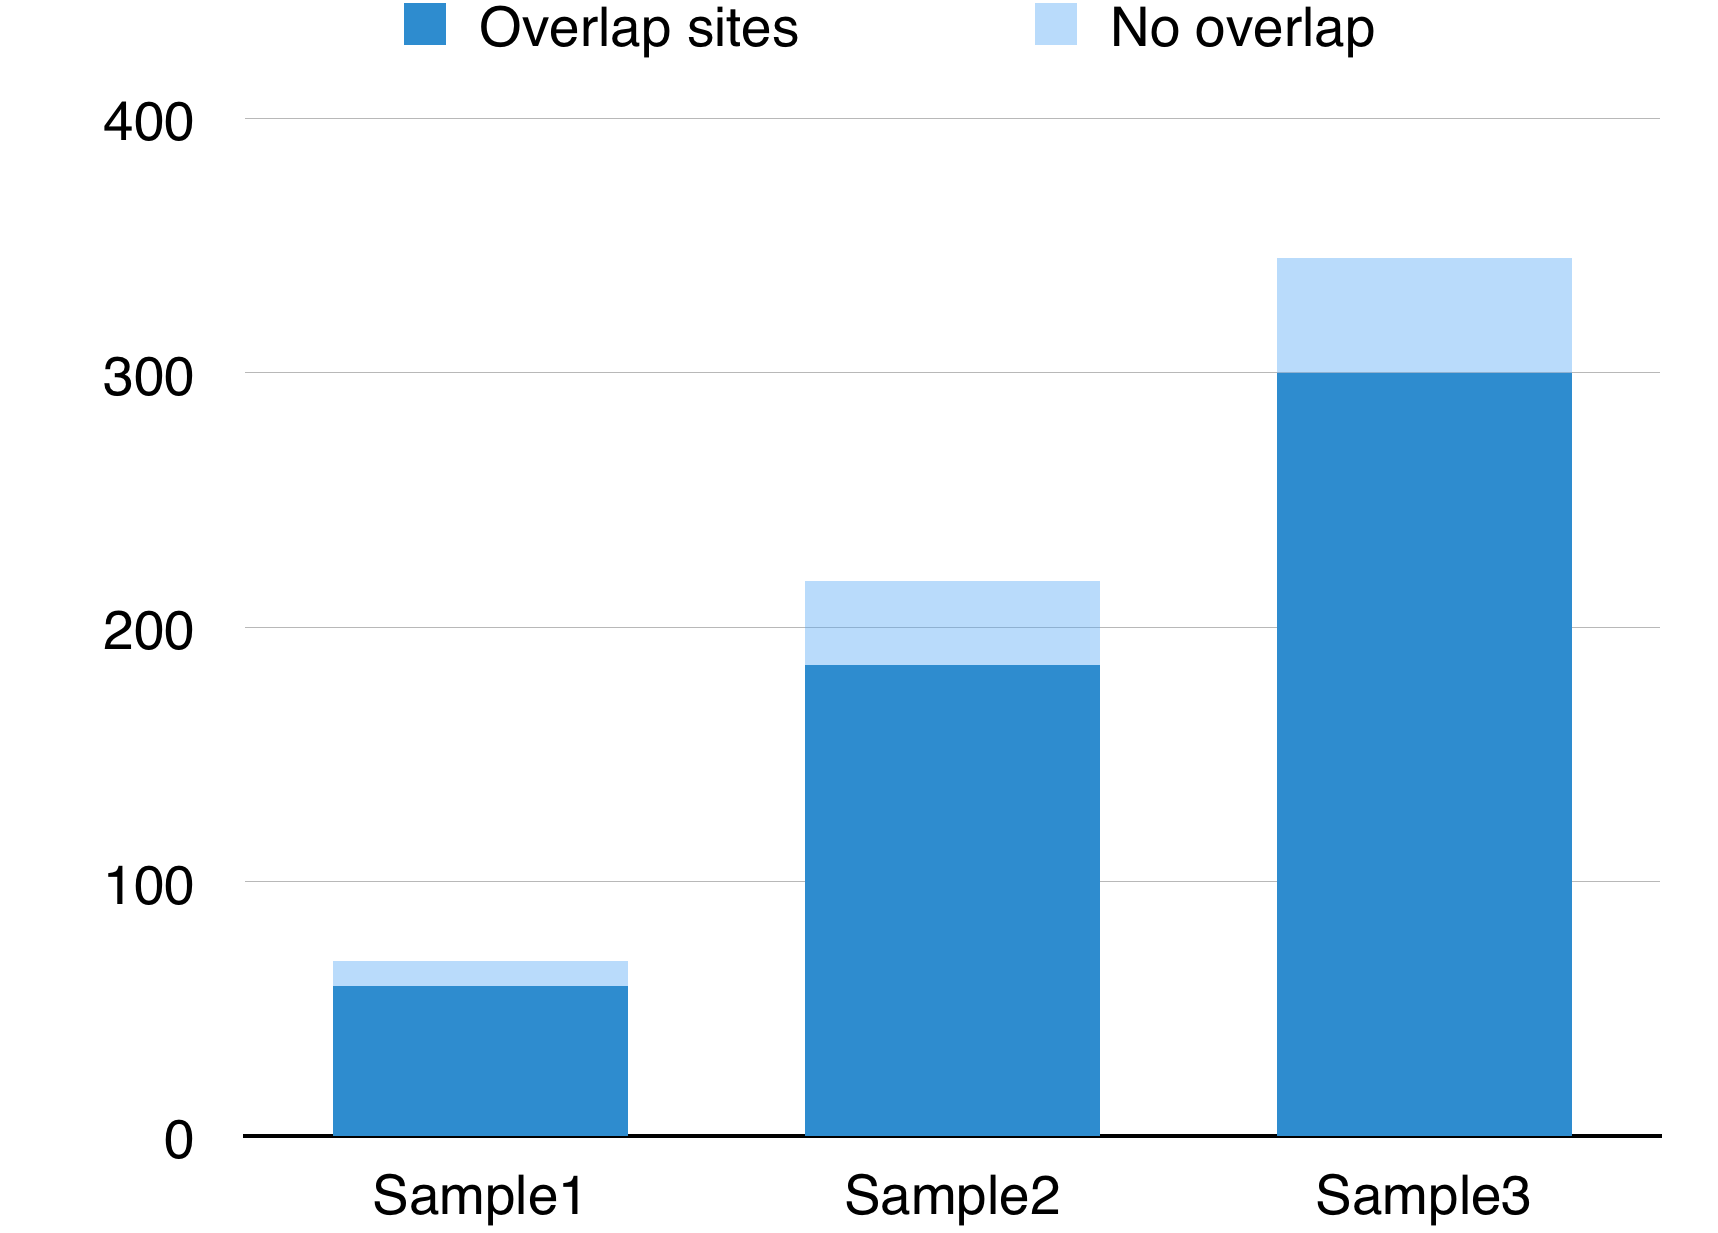
\includegraphics[width=0.5 \hsize]{overlap.png}
	\end{center}
	\caption{追証実験}
	\begin{flushleft}
		\small{追証実験による編集サイトの一致と不一致をそれぞれ表す。}
	\end{flushleft}
	\label{fig:overlap}
\end{figure}

\newpage

\section{議論}
\subsection{本手法により同定された編集サイト}
\subsection{本手法の有用性}
